%Always-Imports
\documentclass[12pt, letterpaper]{article}
\usepackage[utf8]{inputenc}
\usepackage[margin=1in]{geometry}

%Sometimes imports
\usepackage{comment}
\usepackage{graphicx}

%biblatex (as opposed to bibtex) parts
%\usepackage[style=numeric]{biblatex}
%\addbibresource{citations.bib}

\begin{comment}
\usepackage{listings} % Typeset Python
\lstset{breaklines=true}
\end{comment}

\title{COSC 5010-03 (23194) Spring 2023 Project Design Document}
\author{Michael Elgin}
\date{April 2, 2023}

\begin{document}

\maketitle

\section{Purpose}

This design document is for a software application that creates secure data files, such as for journaling or otherwise storing private information. The topic this software addresses is privacy concerns when engaging with technology. With cloud services like OneDrive rising in popularity, there are security concerns with respect to the fact that these cloud services are generally not zero-knowledge cloud systems, i.e. the cloud service provider (such as Microsoft) could read the data and/or transfer it to intelligence agencies. This software will create encrypted journal files, and allow them to be read only by the software application while it is used by a user who possesses the correct password, regardless of where the associated files are kept.

\section{Components}
\subsection{GUI}

The GUI will allow the user to interact with the system visually instead of using a command line. It will allow for interacting with files that are encrypted based on the supplied password. In addition it will give the user create-read-update-delete (CRUD) functionality to all accessible files.

\subsection{Password Security Checker}

This component will provide standard checks on a password to ensure it is secure, such as length, use of numbers/capitals/specials/etc. It will warn the user if their chosen password is insecure on both the terminal and GUI.

\subsection{Middleware}

This connects all the components together. It contains the functions that are called by the GUI. It performs read/write operations on the file system. It handles the cryptography, and bases an encryption key off a hash of a user password.

\subsection{Data Files}

These files will be the data documents which are securely encrypted. At no time will these ever sit at rest on the file system decrypted. They will have their own unique file extension to help identify them on the file system.

\section{Component Interactions}

The GUI will be the starting point of the program; it will launch the middleware and be the main channel of interaction to it, though the middleware could also be interfaced with programmatically. The GUI allows the user to make calls to the middleware through buttons and menus, which in turn interacts with the password security checker and the datafiles. Middleware interacts with the password security checker by importing it. Middleware interacts with datafiles through file system read/write operations.
The GUI, password security checker, and data files have no direct interactions between themselves; they are completely mediated by the middleware.

\section{Security Challenges and Assumptions}

\subsection{Challenges}
The first challenge is privacy design. It must be that the contents of data files are kept secret. If a data file is acquired by anyone other than someone who has the password, it should not be readable. A second challenge is to help ensure the passwords created by the user are secure i.e. they do not choose passwords that would be easily guessed, brute-forced, or otherwise learned by an attacker. A third challenge is that the encryption key must be based off the password in a secure way. There should be no shortcuts from the password to the key.

\subsection{Assumptions}
One assumption as per Kerckhoff's principle is that the software itself, including its code, need not be hidden. The same instance of it could securely be used by multiple different users, even in the same working directory, so long as passwords are kept secret. A second assumption is that the cryptography library will also ensure integrity with message authentication codes.

This software is not a distributed system, and the security concerns of a distributed system are not relevant here. However, if a data file were to be sent across a network, it should still be secure by virtue of its encryption.

\section{Addendum April 26, 2023 - 5010 Extension}

\subsection{High-level proof sketch}

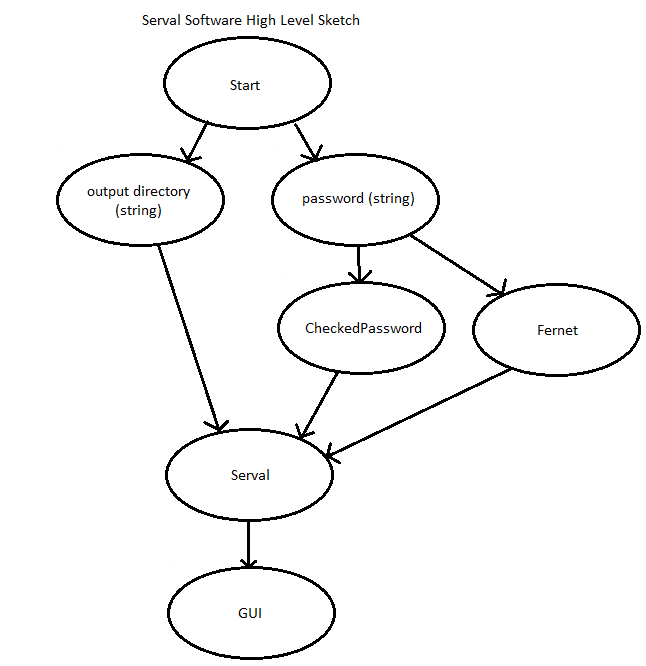
\includegraphics[scale=0.6]{High_Level_Proof_Sketch.png}

\subsection{External threats}

One possible threat from an attacker is to change the contents of a .serval file. Though because of the HMAC built into the fernet tokens, this will be detected and an InvalidToken exception will be thrown. Handling this exception and type checking that the returned contents are None will prevent such meddling from being passed through the chain of execution.

\subsection{The system being run on}

The software is designed and expected to be portable to any system that can run Python 3.11. As such it makes no mention of any particular operating system or hardware. One threat is that the system may mishandle .serval files. The use of types is meant to ensure that no matter how any underlying system may mishandle the storage of .serval files, the software always receives the proper type to operate on. 

\subsection{Threats created by interfacing}

The most prominent threat created by interfacing is the possibility that someone could construct a Serval object and pass bad input to its methods. In the case of the function to set the checked password, the object passed will cause an exception unless it is something that can be converted into a string and checked as such. When setting any output directory, any type that does not resolve to a string that is a valid directory path on the file system will cause the function to return False as it should. The CRUD functions are a similar case since they present no security hazards from wrong types.

For CheckedPassword objects, the check function presents no risks from wrong types, as does the way user-friendly warnings are gathered, since if the input does not resolve to certain strings in a mapping there will be a keyError exception.

Programmatically specifying bad input could cause an exception to be thrown, but it should not cause any security hazards.

Another threat is that different versions of dependencies may return different types. To help reduce the chance that any differences in dependency version cause a return of different types, specific versions of dependencies are listed in the README.md and are considered a recommendation.

\end{document}